\chapter{Contributions} \label{chap:Contributions}


\section*{Introduction}
With the birth of the smart grid as the next step of evolution for grid infrastructure, with the improvements that the smart grid came with, like improved reliability, automation, and faster detection and response to failures, it also came with its own set of risks and disadvantages. mainly due to the fact that it is composed of multiple components and systems that are connected to the internet, like wireless networks and sensors, smart meters, and IoT devices, making it an easy target for hackers. independent groups or state actors whose goal is to cause as much damage as possible or to collect valuable data. On top of those components, there are legacy systems that the smart grid relies on that are known for their many and major security vulnerabilities, which are all easy targets, for example, Supervisory Control and Data Acquisition (SCADA). As an example of those risks and weaknesses, we can look at the situation Ukraine found itself in after Russia targeted their smart grid systems in 2015, leaving 80,000 Ukrainian households without power for 3 to 6 hours. \cite{ukrain-sg-attack}.

That's why it is important to protect the smart grid system from cyberattacks by employing IDS, IPS, and IDPS. 
as the second line of defense in case encryption and authorization were unsuccessful in stopping the cyberattack from targeting the smart grid system.

\newpage




\section{Intrusion detection systems (IDS)}
An intrusion detection system is a piece of hardware or software that is responsible for detecting suspicious and malicious activity, and in a network or an information system, the anomaly can either be reported to a systems administrator or saved to a security information and even management system (SIEM), the SIEM combines the output from multiple sources, then uses some filtering techniques to decide if the reported activity is malicious. \cite{ids-def}
An IDS on its own cannot stop intrusions; it can only detect and report them. However, with its evolution, the intrusion prevention system (IPS) or intrusion detection and prevention system (IDPS) can counter an attack. \cite{ibm-ids}








\section{Intrusion detection systems architecture}
Intrusion detection systems, like any complex system, are made of multiple interoperating components with a specific task assigned to each component. Although the functioning of an IDS changes vastly between different types of IDSs (diffrent in deployment or detection methods), they all share a common general architecture, which is composed of the following components as shown in Figure \ref{fig:arch_IDS} \cite{arch-IDS}:

\begin{figure}[h]
	\centering
	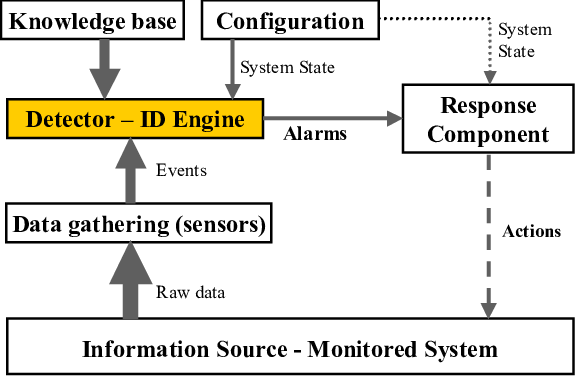
\includegraphics[width=400px]{figures/arch_IDS.png}
	\caption{IDS architecture \cite{arch-IDS}}
	\label{fig:arch_IDS}
\end{figure}

\firmlist
\begin{itemize}
	\item Data gathering components (sensor): tasked with collecting information from the monitored environment.
	\item Detector (IDS engine): analyzes the data collected by the sensor to determine the presence of suspicious activity.
	\item Knowledge base(database): the database that stores information collected previously by sensors about known attacks that allows the engine to determine the suspesious activity.
	\item Configuration component: defines settings and the behavious of the system.
	\item Response component: this component is responsible for responding to the detected intrusion and either attempts to prevent the intrusion (IPS) or reports it to a human administrator (IDS).
\end{itemize}



\section{Intrusion detection systems classification}
Intrusion detection systems are classified according to two criteria of classification, which are as shown in Figure \ref{fig:IDS-classification-taxonomy} are:

\firmlist
\begin{itemize}
	\item deployment method
	\item detection method
\end{itemize}

\cite{ids-classification}


\begin{figure}[h]
	\centering
	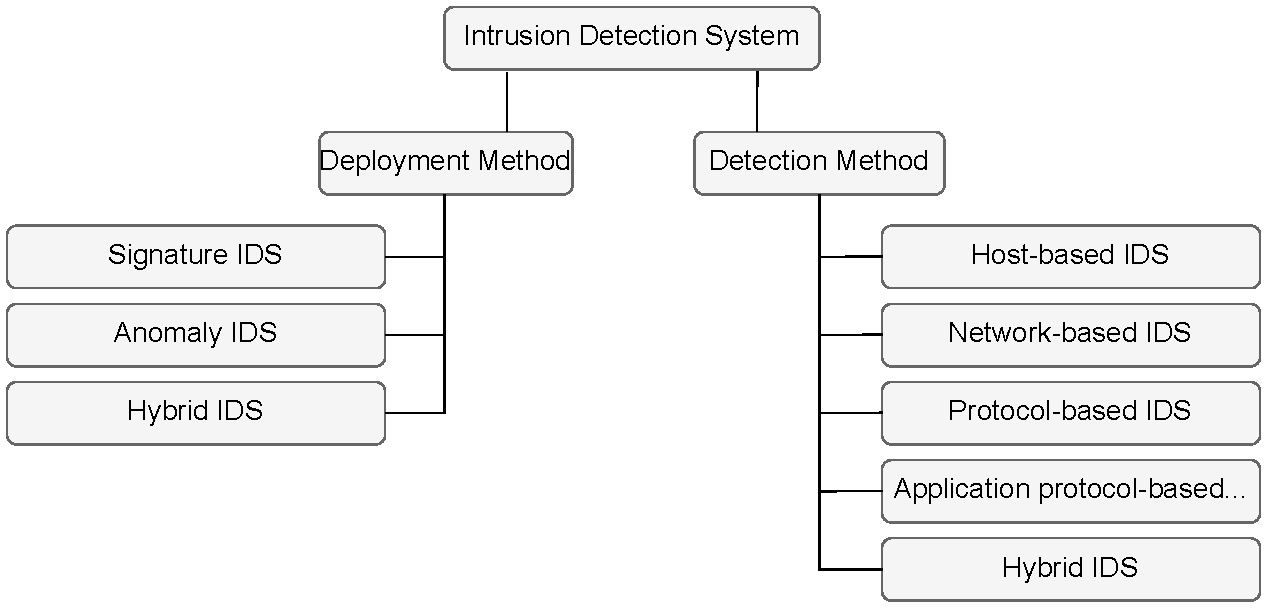
\includegraphics[width=400px]{figures/IDS_classification.pdf}
	\caption{IDS classification taxonomy}
	\label{fig:IDS-classification-taxonomy}
\end{figure}




\subsection{Deployment methods}

2 primary are HIDS and NDIS 

some more specialized methods PIDS APIDS and hybrid
https://www.ibm.com/topics/intrusion-detection-system


\subsubsection{NIDS}
Network intrusion detection systems are the most commonly used commercial IDS. They are usually placed at the start edge of the sub-network, right after the firewall (if one exists), so they can have access to all inbound traffic to all devices on the network \cite{NIST-IDS}. NIDS protects the networks from cyber attacks and threats by scanning and monitoring TCP/IP packets for known attack signatures and reporting them to the administrator \cite{NIDS-ip-tcp}

Some benefits of using a NIDS are that a few well-placed NIDS can be enough to cover an entire large network. In addition, their deployment requires minimal refactoring of the network, meaning easy installation \cite{NIST-IDS}. But the downsides are that they cannot detect threats with inaccurately constructed attack signatures and cannot analyze encrypted traffic, and it is hard to work with networks operating at 10 Gbps \cite{NIDS-ip-tcp}.

With a NIDS, one would ideally scan all inbound and outbound traffic; however, doing so might create a bottleneck that would impair the overall speed of the network.


\begin{figure}[h]
	\centering
	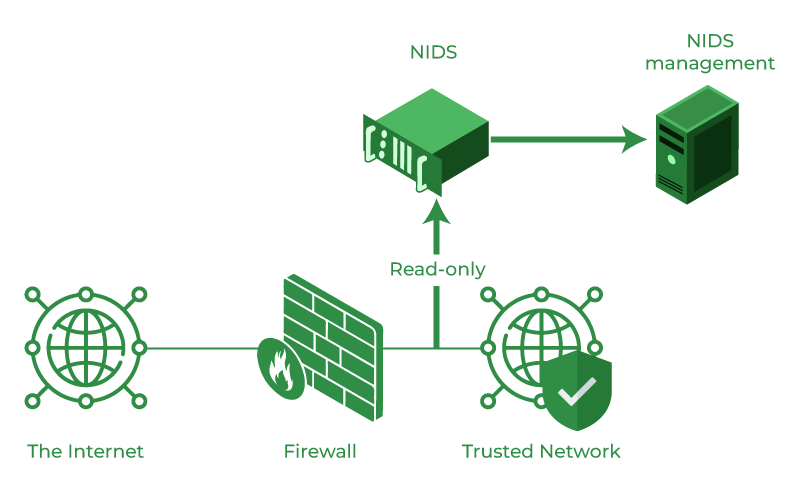
\includegraphics[width=300px]{figures/NIDS.png}
	\caption{NIDS \cite{geeksforgeeks}}
	\label{fig:NIDS}
\end{figure}



\subsubsection{HIDS}
Unlike NIDS, HIDS run on individual devices in a network, making it's threat detection scope more focused. They monitor all incoming and outgoing traffic and alert the administrator if suspicious or malicious activity is detected.

It is considered to be more reliable than NIDS because it has access to files in the operating system, and it can detect if a file has been tampered with by keeping snapshots of previous versions of those system files and comparing them to the current version to decide if it has been tampered with. \cite{NIST-IDS}

This type of IDS uses 2 sources of information inside the device's operating system:

\firmlist
\begin{itemize}
	\item system audit trails: operating system audit trails are created by the kernel making them very detailed because the kernel has access to everything in an OS. \cite{NIST-IDS}
	\item system logs: less complex the system audit trails making them easier to understand. \cite{NIST-IDS}
\end{itemize}



\begin{figure}[h]
	\centering
	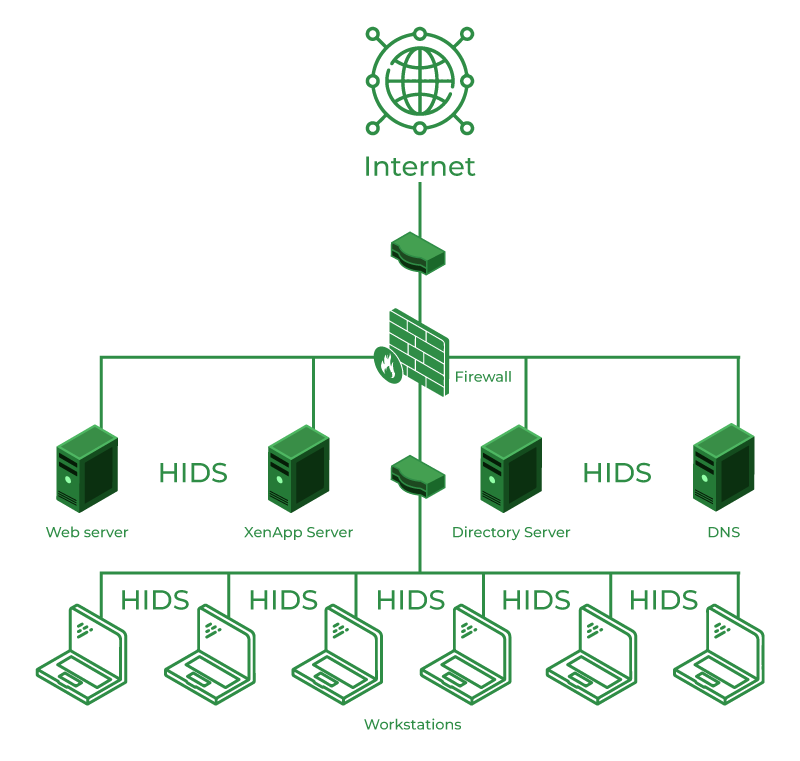
\includegraphics[width=300px]{figures/HIDS.png}
	\caption{HIDS \cite{geeksforgeeks}}
	\label{fig:HIDS}
\end{figure}



\subsubsection{Other types of IDS}
uncommon types with specific functions usally used togther with NIDS or HIDS to augment thier detection capabilities

\firmlist
\begin{itemize}
	\item Protocol intrusion detection system (PIDS): this type of IDS monitors the protocol in use (like HTTP or HTTPS) between the server and the client. PIDS is usually placed at the front end of the server. \cite{geeksforgeeks}


	\item Application protocol detection system (APIDS): specialized in application security, it analyzes the packets of application-specific protocols (like MySQL) to determine the presence of suspicious activity. APIDS are usually placed on groups of servers. \cite{geeksforgeeks}
	

	\item hybrid detection system: it is a combination of two or more of any of the previously defined IDSs. It is more reliable than any individual IDS because it has access to the data accessible to all of the used IDSs, providing it with a network-wide view.
	\cite{geeksforgeeks}
\end{itemize}




\subsection{Detection methods}
there are 2 primary methodes of detection for IDS which are anomaly-based and signature-based (which is also known as misuse intrusion detection or knowledge-based intrusion detection). \cite{ids-classification}



\subsubsection{Signature-based detection}
SIDs define patterns in known cyberattacks and store them in a database as signatures. The SID then analyzes system activity and search for a pattern of suspicious activity that matches previously documented attacks's signatures. This method provides high detection capabilities against known attacks. even though it cannot detect new attacks. On top of that, the database of previous attacks is very large, and having to compare internet packets to this database is resource- and time-consuming. \cite{NIST-IDS}



\subsubsection{Anomaly-based detection}
AIDs can identifi abnormal behavious in the enviroment it is used in, this type of IDS first observes and models the normal behaviours then compares the trffic to this model to determine the presnece of suspesious activity. the constructed model is created based on the data collected by observing the behaviour of the system over a specific period of time of normal operation. \cite{NIST-IDS}

AIDs often lead to a lot of false negatives because the normal activity varies alot over time, althout it is better than SIDs in detecting new and unknown attacks. it can also be used to provide new data for the signature-based detection systems. \cite{NIST-IDS}




\subsubsection{Hybrid detection}
is in development
\clearpage

\subsubsection{Signature-based VS Anomaly-based detection}
table of pros and cons
sigVSano.tex
\begin{table}[h]
	\centering
	\caption{An example of tables}
	\begin{tabular}{|L{1.2cm}C{7cm}R{7cm}|}  % sum=15.2cm (L=Left, C=Center, R=Right)
	\hline
	& Signature-based & Anomaly-based \\
	Pros &
	\firmlist
	\begin{itemize}
		\item simple and effective against know attacks
		\item fewer false positives
	\end{itemize}
	&
	\firmlist
	\begin{itemize}
		\item Ineffecitve againts new and unknown attacks
		\item slow if the database is large
		\item database needs to be cosntantly constanlty maintained and updated
	\end{itemize}
	\\

	Cons &
	\firmlist
	\begin{itemize}
		\item can detect new and unknown attacks
		\item can provide data to Signature-based detection
	\end{itemize}
	&
	\firmlist
	\begin{itemize}
		\item more false negatives
		\item needs training to build normal behaviour models
	\end{itemize}
	\\
	\hline
\end{tabular}
	\label{tab:example}
\end{table}




\section{Evolutions of IDS: IPS/IDPS}
The biggest disadvantage of an IDS is its inability to react to attacks and actively block malicious activity. That's why it was necessary to create a new system to overcome those drawbacks, which is IPS, also known as IDPS.

IPS types
- NIPS
- WIPS
- HIPS
- NBA

IPS detection methodes
- signature based
- statistical anomaly based
- stateful protocol abalasys 


\section{maybe IDS usage in smart grid}
required to be able to do :
- detecting wide range of intrusions
- fast detection
- accuracy (FP/FN/TP/TN)
- resource effecient
- scalable
- easy to operate (user friendly)


\subsection{maybe IDS requirements}

\subsection{maybe IDS importance}


\section{conclusion}













\chapter{Implementation} \label{chap:Implementation}
